\section{Problem 2D: Stochastic SEIIaR Commuter model}

\subsection{a) Commuter model for a two-town system}

I set up a population structure as described by the matrix 
$$
	\mathbf{M} = \begin{bmatrix}
	9000 & 1000 \\
	200 & 99800
	\end{bmatrix},
$$
and simulate the time evolution of each of the five states for $180$ days, as described in \cite{sheet}, with $25$ initially exposed people working and living in town $1$. The results of this simulation is shown in figure \ref{fig:commuter_2city}. Notice that we here use the number of people as scale on the vertical axis, so that we easier can distinguish the two towns from each other. We observe that the evolution of the epidemic in town $2$ is delayed compared to that of town $1$. This is as expected, as only $25$ people in town $1$ are exposed, and they can only infect people in town $2$ \textit{via} someone that works in town $2$ during the night, or someone that works in town $1$ while living in town $2$ during daytime. 

Also here, note that at each time there are fewer asymptomatic infected than symptomatic infected. This is as expected since $f_a < f_s$, and $r_a < r_s$.

\begin{figure}[htb]
	\centering
	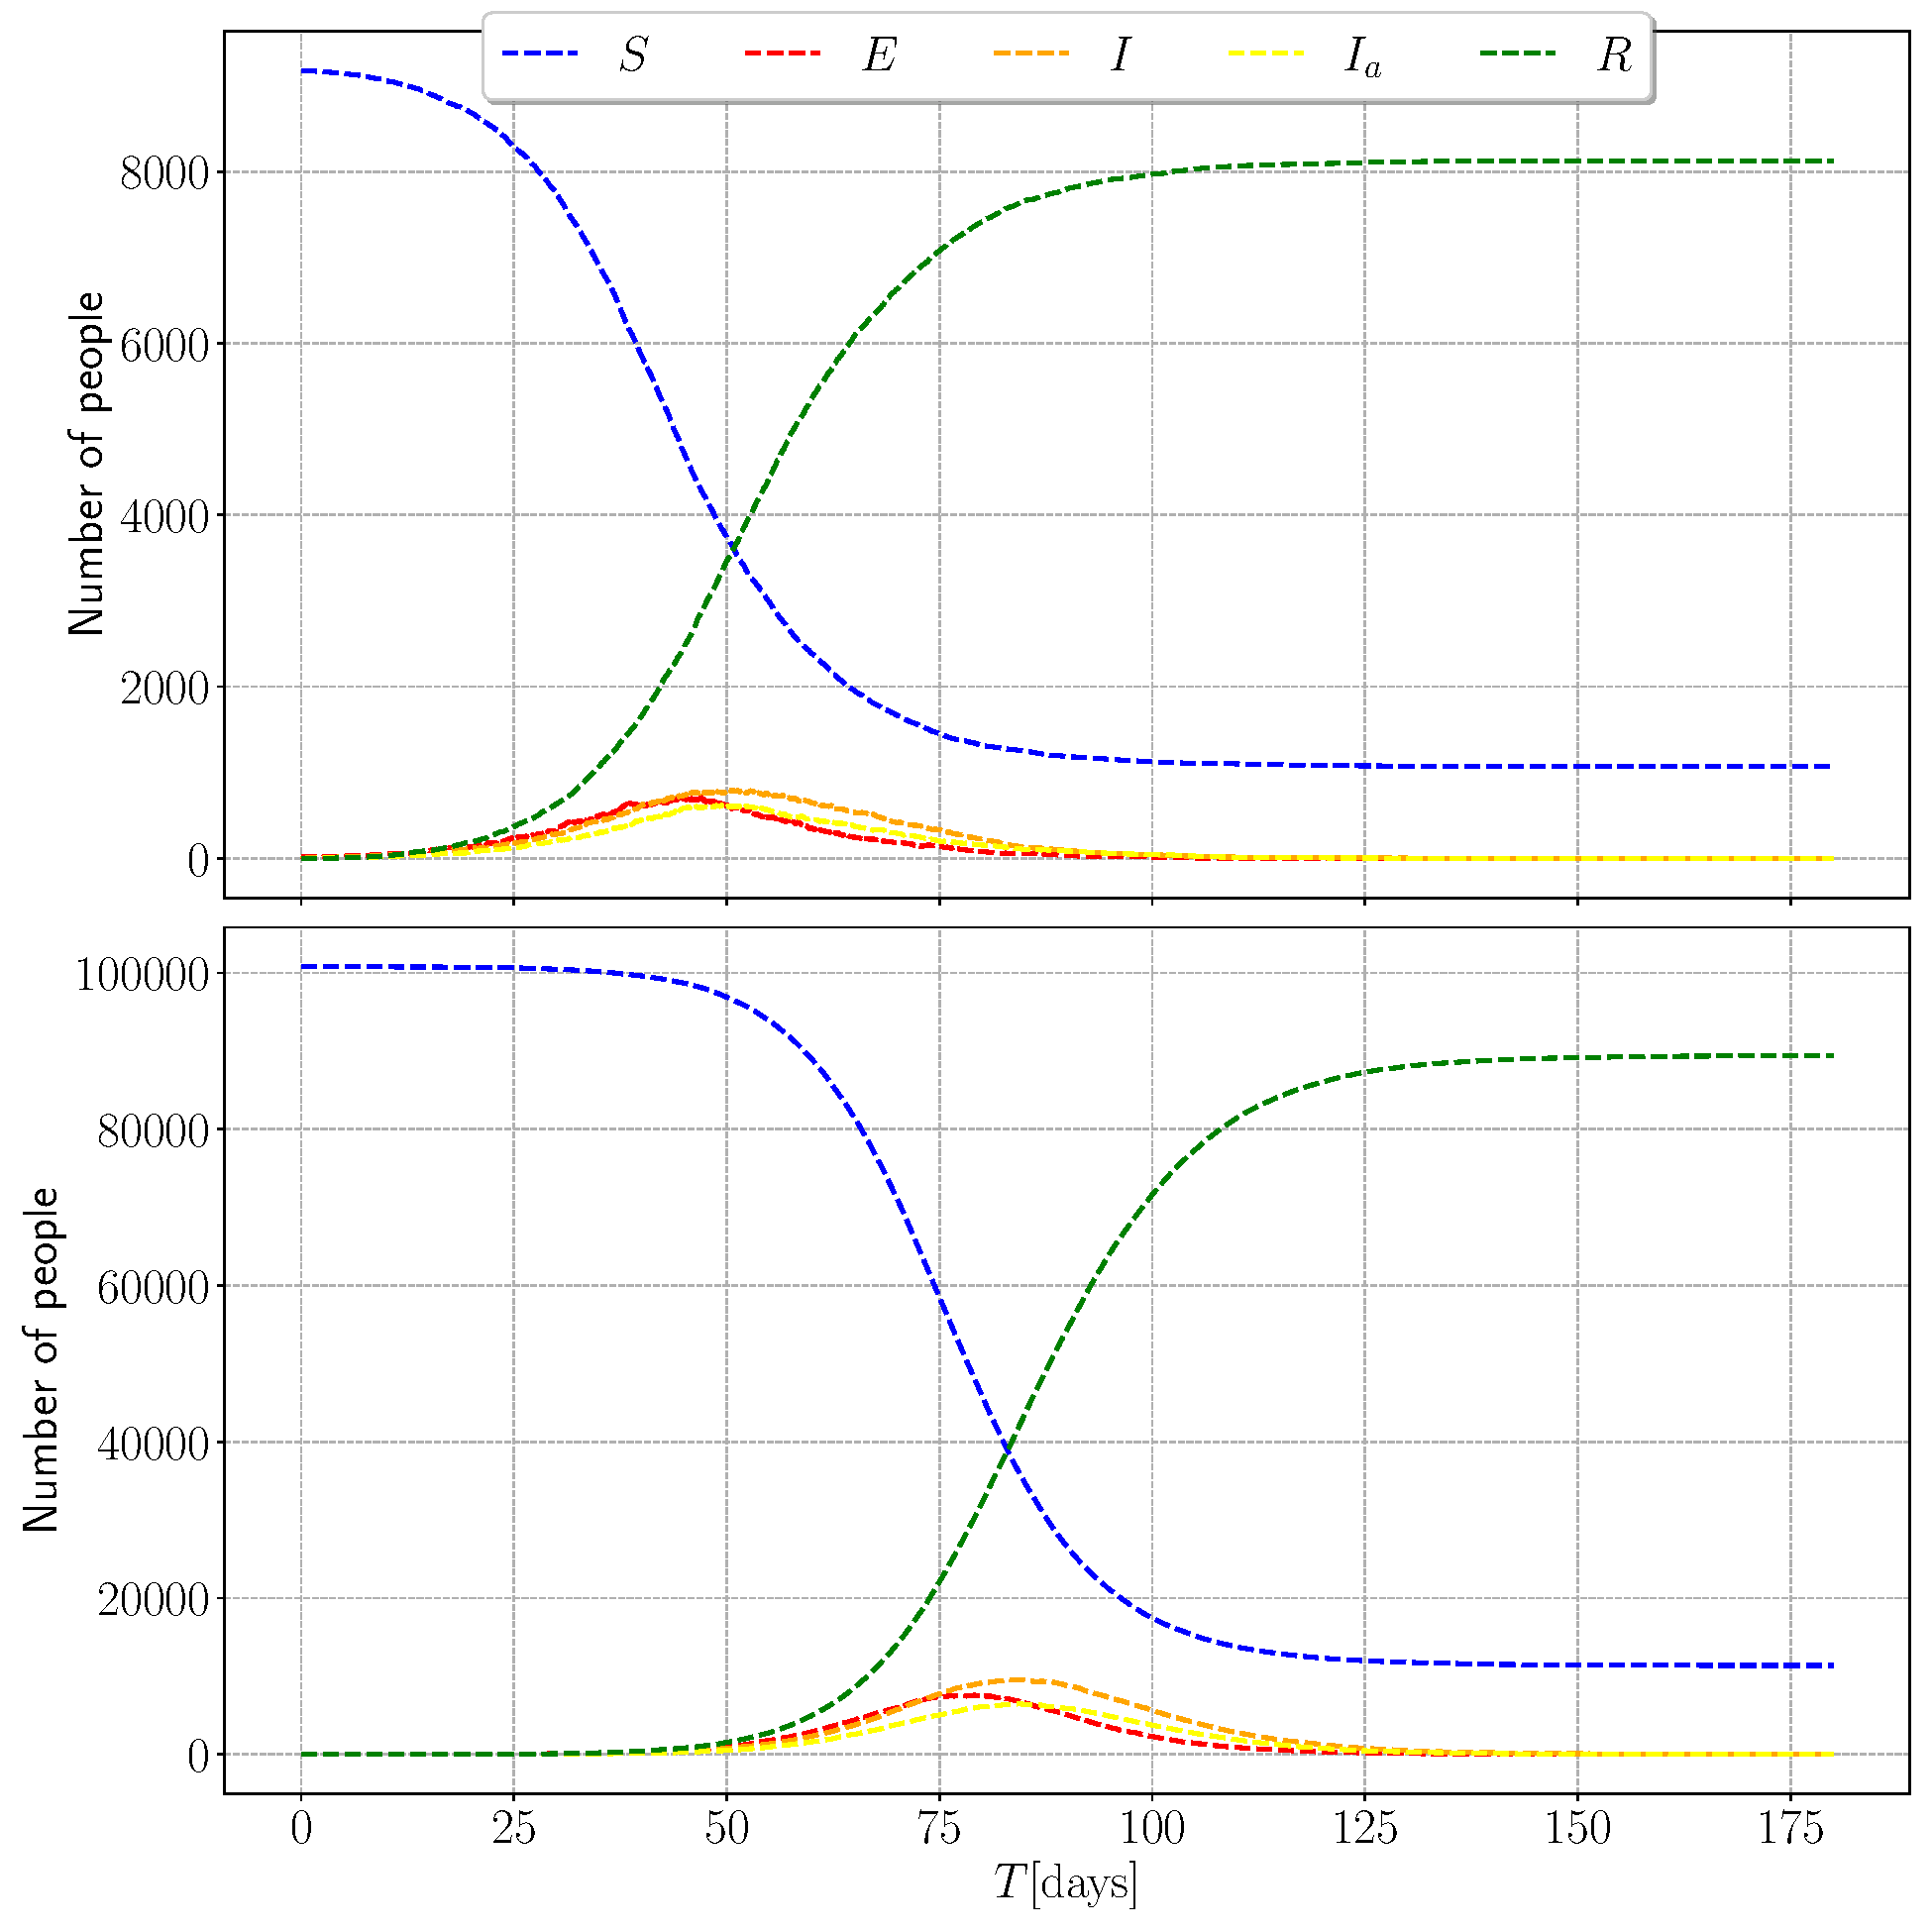
\includegraphics[width=0.8\columnwidth]{../fig/2Da_commuter.pdf}
	\caption{Solutions of Stochastic SEIIaR commuter model for the $2$-city case.}
	\label{fig:commuter_2city}
\end{figure}

\subsection{b) Description of implementation \& tests} 

To implement the Stochastic SEIIaR Commuter model, I choose the following procedure: 

\begin{algorithm}[H]
	Choose a population structure $\mathbf{M} \in \mathbb{N}^m \times \mathbb{N}^m$, i.e. an $m\times m$ matrix\;  
	Set an end time $t_N$ and a time-step $\Delta t$\;
	Set an initial state $\mathbf{X}_0 \in \mathbb{N}^m \times \mathbb{N}^m \times \mathbb{N}^5$, where entry $X_{0,ij}$ is the vector $\mathbf{v}$ of the variables $S,E,I,I_a,R$ for group $(i,j)$ in the matrix $\mathbf{M}$.\;
	Create an empty array for holding the state at each point in time, $\mathbf{X}$, and set its first element to $\mathbf{X}_0$.\;
	Calculate the probabilities:
	\begin{align*}
		P_{E\to I} &= f_s \times (1 - \exp{(-\Delta t/\tau_E)}) \\
		P_{E\to I_a} &= f_a \times (1 - \exp{(-\Delta t/\tau_E)}) \\
		P_{I\to R} = P_{I_a\to R} &= 1 - \exp{(-\Delta t/\tau_I)} 
	\end{align*}
	Calculate the number of days $D = \texttt{int}(t_N)$, and the number of steps per half day $S = \texttt{int}(1/(2\Delta t))$.\; 
	\For{$d = 0,\dots, D - 1$}
		{
		$i \gets 2 \times d \times S$\;
		\For{$j = 0,\dots, S - 1$}
			{
			Calculate the number of people in each town, $\beta$,
				$$
				N_\beta = \sum_{\alpha = 1}^{m} M_{\alpha \beta} 
				$$ 
			Find the number of infected people of each kind at the previous time step for each town $\beta$,
				$$
				I_{\beta}, I_{a,\beta} = \sum_{\alpha = 1}^{m} X_{(i+j)\alpha\beta3},  \sum_{\alpha = 1}^{m} X_{(i+j)\alpha\beta4} 
				$$
			Calculate the probability for transitioning between $S$ and $E$ for each town, $\beta$, \footnote{Note that here I have used $\beta_0$ to denote the beta value describing the value of the model, to not confuse it with the summation variables.}
				$$
				P_{S\to E,\beta} = 1 - \exp{\left( - \Delta t \beta_0 \frac{r_s I_{\beta} + r_a I_{a,\beta}}{N}\right)} 
				$$
			}
			Do a normal SEIIaR step for each group of people $\alpha,\beta = 1,\dots,m$, exactly as described in the introduction to update to the present state $X_{(i+j+1)\alpha\beta\gamma}$\;   
		$i \gets i + S$\;
		\For{$j = 0,\dots, S - 1$}
			{
			Repeat the procedure in the loop above, but with $\alpha \leftrightarrow \beta$, i.e. perform the sums over the \textit{third} not \textit{second} axis of $\mathbf{X}$, and the \textit{second} of $\mathbf{M}$. \;
			}
		}
		\caption{Description of implementation of the SEIIaR commuter model.}
\end{algorithm} 

Listing \ref{lst:commuter} shows the same algorithm as described above implemented in python.

\begin{lstlisting}[language=Python,label={lst:commuter},caption={SEIIaR commuter algorithm implemented in python}]
@nb.njit()
def SEIIaR_commuter_step(X,Pse,Pei,Peia,Pir,Piar):

    Dse          = np.random.binomial(X[0],Pse)
    Dei,Deia,Dee = np.random.multinomial(X[1], (Pei,Peia,1-Pei-Peia) )
    Dir          = np.random.binomial(X[2], Pir)
    Diar         = np.random.binomial(X[3], Piar)

    return np.array([X[0] - Dse,
                     X[1] - Dei - Deia + Dse,
                     X[2] - Dir + Dei,
                     X[3] - Diar + Deia,
                     X[4] + Dir + Diar])

@nb.njit()
def SEIIaR_commuter(M,X_0,tN,dt):
    
    # set this to ones initially, but change it 
    # for each step, as it depends on the number of infected.

    m    = np.shape(M)[0] 
    Pse  = np.ones(m)

    Pei  = fs * (1 - np.exp(-dt/tau_E))
    Peia = fa * (1 - np.exp(-dt/tau_E))
    Pir  = 1 - np.exp(-dt/tau_I)
    Piar = 1 - np.exp(-dt/tau_I)

    T = np.arange(0,tN+dt,dt)
    n = len(T)

    X          = np.zeros((n,m,m,5),dtype = np.int64)
    X[0,:,:,:] = X_0

    # The loop below assumes that the simulation is
    # runned for a whole number of days, with 0.5 divisible by dt,
    # so that the number of steps are evenly split into night and day.
    
    assert( int(0.5 / dt) * dt  == 0.5 )

    step_length = int(1/(2*dt))
    days       = int(tN)
    
    for day in range(days):

        i = day * 2 * step_length # current start index
        
        for j in range(step_length):

            # Daytime simulation
            
            N = np.sum(M,axis = 0)
            I = X[i+j,:,:,2:4]
            I = np.sum(I, axis = 0)
            Pse = 1 - np.exp(- dt * beta * 1/N * ( rs * I[:,0] + ra * I[:,1] ))
            for k in range(m):
                for l in range(m):
                    X[i+j+1,k,l,:] = SEIIaR_commuter_step(X[i+j,k,l,:],Pse[k],Pei,Peia,Pir,Piar)

        i += step_length

        for j in range(step_length):

            # Night simulation 
            
            N = np.sum(M,axis = 1)
            I = X[i+j,:,:,2:4]
            I = np.sum(I, axis = 1)
            Pse = 1 - np.exp(- dt * beta * 1/N * ( rs * I[:,0] + ra * I[:,1] ))
            for k in range(m):
                for l in range(m):
                    X[i+j+1,l,k,:] = SEIIaR_commuter_step(X[i+j,l,k,:],Pse[k],Pei,Peia,Pir,Piar)

    return T, X
\end{lstlisting}

To check that the system behaves as expected, we simulate the same scenario, only with another matrix which now represents \textit{no} flow of workers to the other areas during daytime:
\begin{equation}\label{eq:test_matrix}
	\mathbf{\widetilde{M}} = \begin{bmatrix}
		10000 & 0 \\
		0 & 100000 
	\end{bmatrix}.
\end{equation}

The time-evolution of the different variables are shown in figure \ref{fig:test_commuter}, in which it is apparent that the exposed people in the small city never infect those in the large city, as we expect. Furthermore, we see that the epidemic in area $1$ evolves slower in this case --- the peak of the infected is delayed by approximately $25$ days. This is also as expected, since more potential carriers of infection are available when the two towns mix during daytime. The expected behaviour is also observed when the exposed start out in area $2$, but a plot of this is not included, for brevity. 

To do a second test we let $9999$ of the people living in town $1$ work in town $2$, and leave only one working in town $1$\footnote{The reason I leave one worker in town $1$ is that having $0$ people in area $1$ at daytime makes the solver break down, as we divide by $0$ in the expression for $P_{S\to E}$}. That is, we use the population matrix in equation \eqref{eq:test_matrix_2}
\begin{equation}\label{eq:test_matrix_2}
	\mathbf{\overline{M}} = \begin{bmatrix}
		1 & 9999 \\
		0 & 100000 
	\end{bmatrix}.
\end{equation}
We simulate the same situation, with $25$ of the $9999$ people initially exposed. This should make the evolution of the variables approximately in sync. This is indeed what we observe, in figure \ref{fig:test_commuter_2}, as the number of infected people in each town are closely synced.

\begin{figure}[htb]
	\centering
	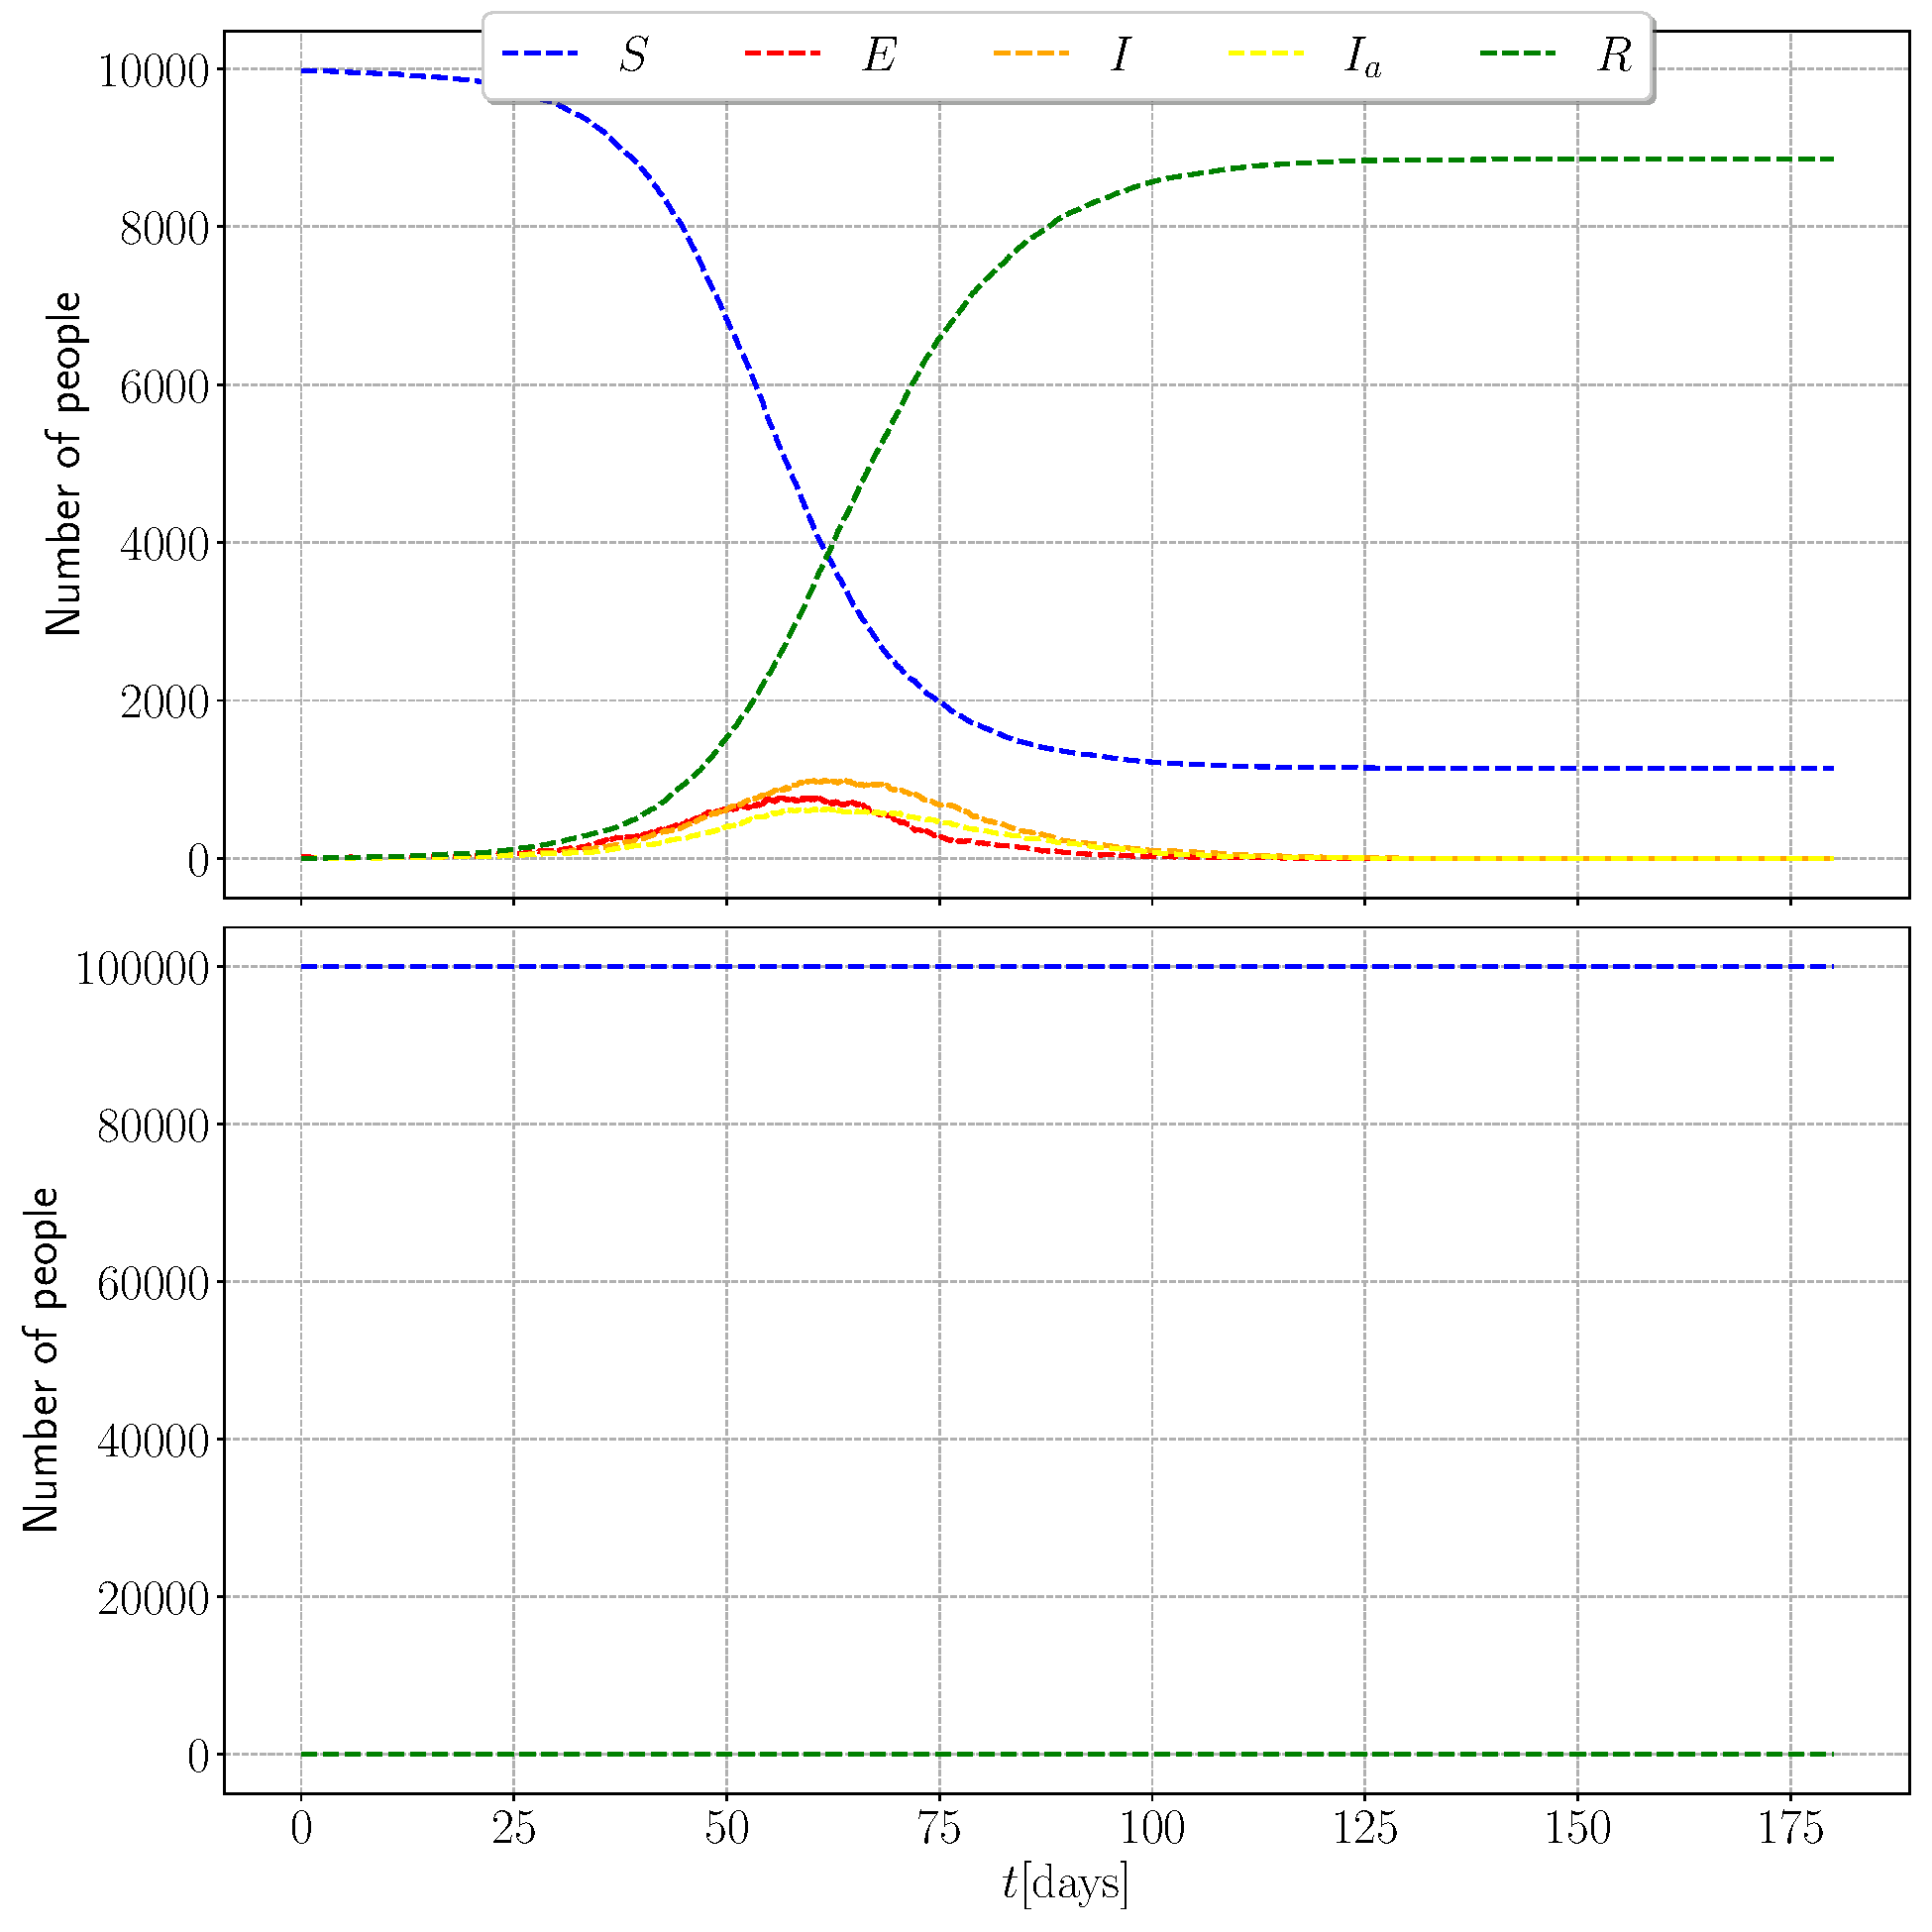
\includegraphics[width=0.6\columnwidth]{../fig/test_commuter.pdf}
	\caption{Solutions of Stochastic SEIIaR commuter model for the $2$-city case, with the matrix $\mathbf{\widetilde{M}}$ in equation \eqref{eq:test_matrix}.}
	\label{fig:test_commuter}
\end{figure}

\begin{figure}[htb]
	\centering
	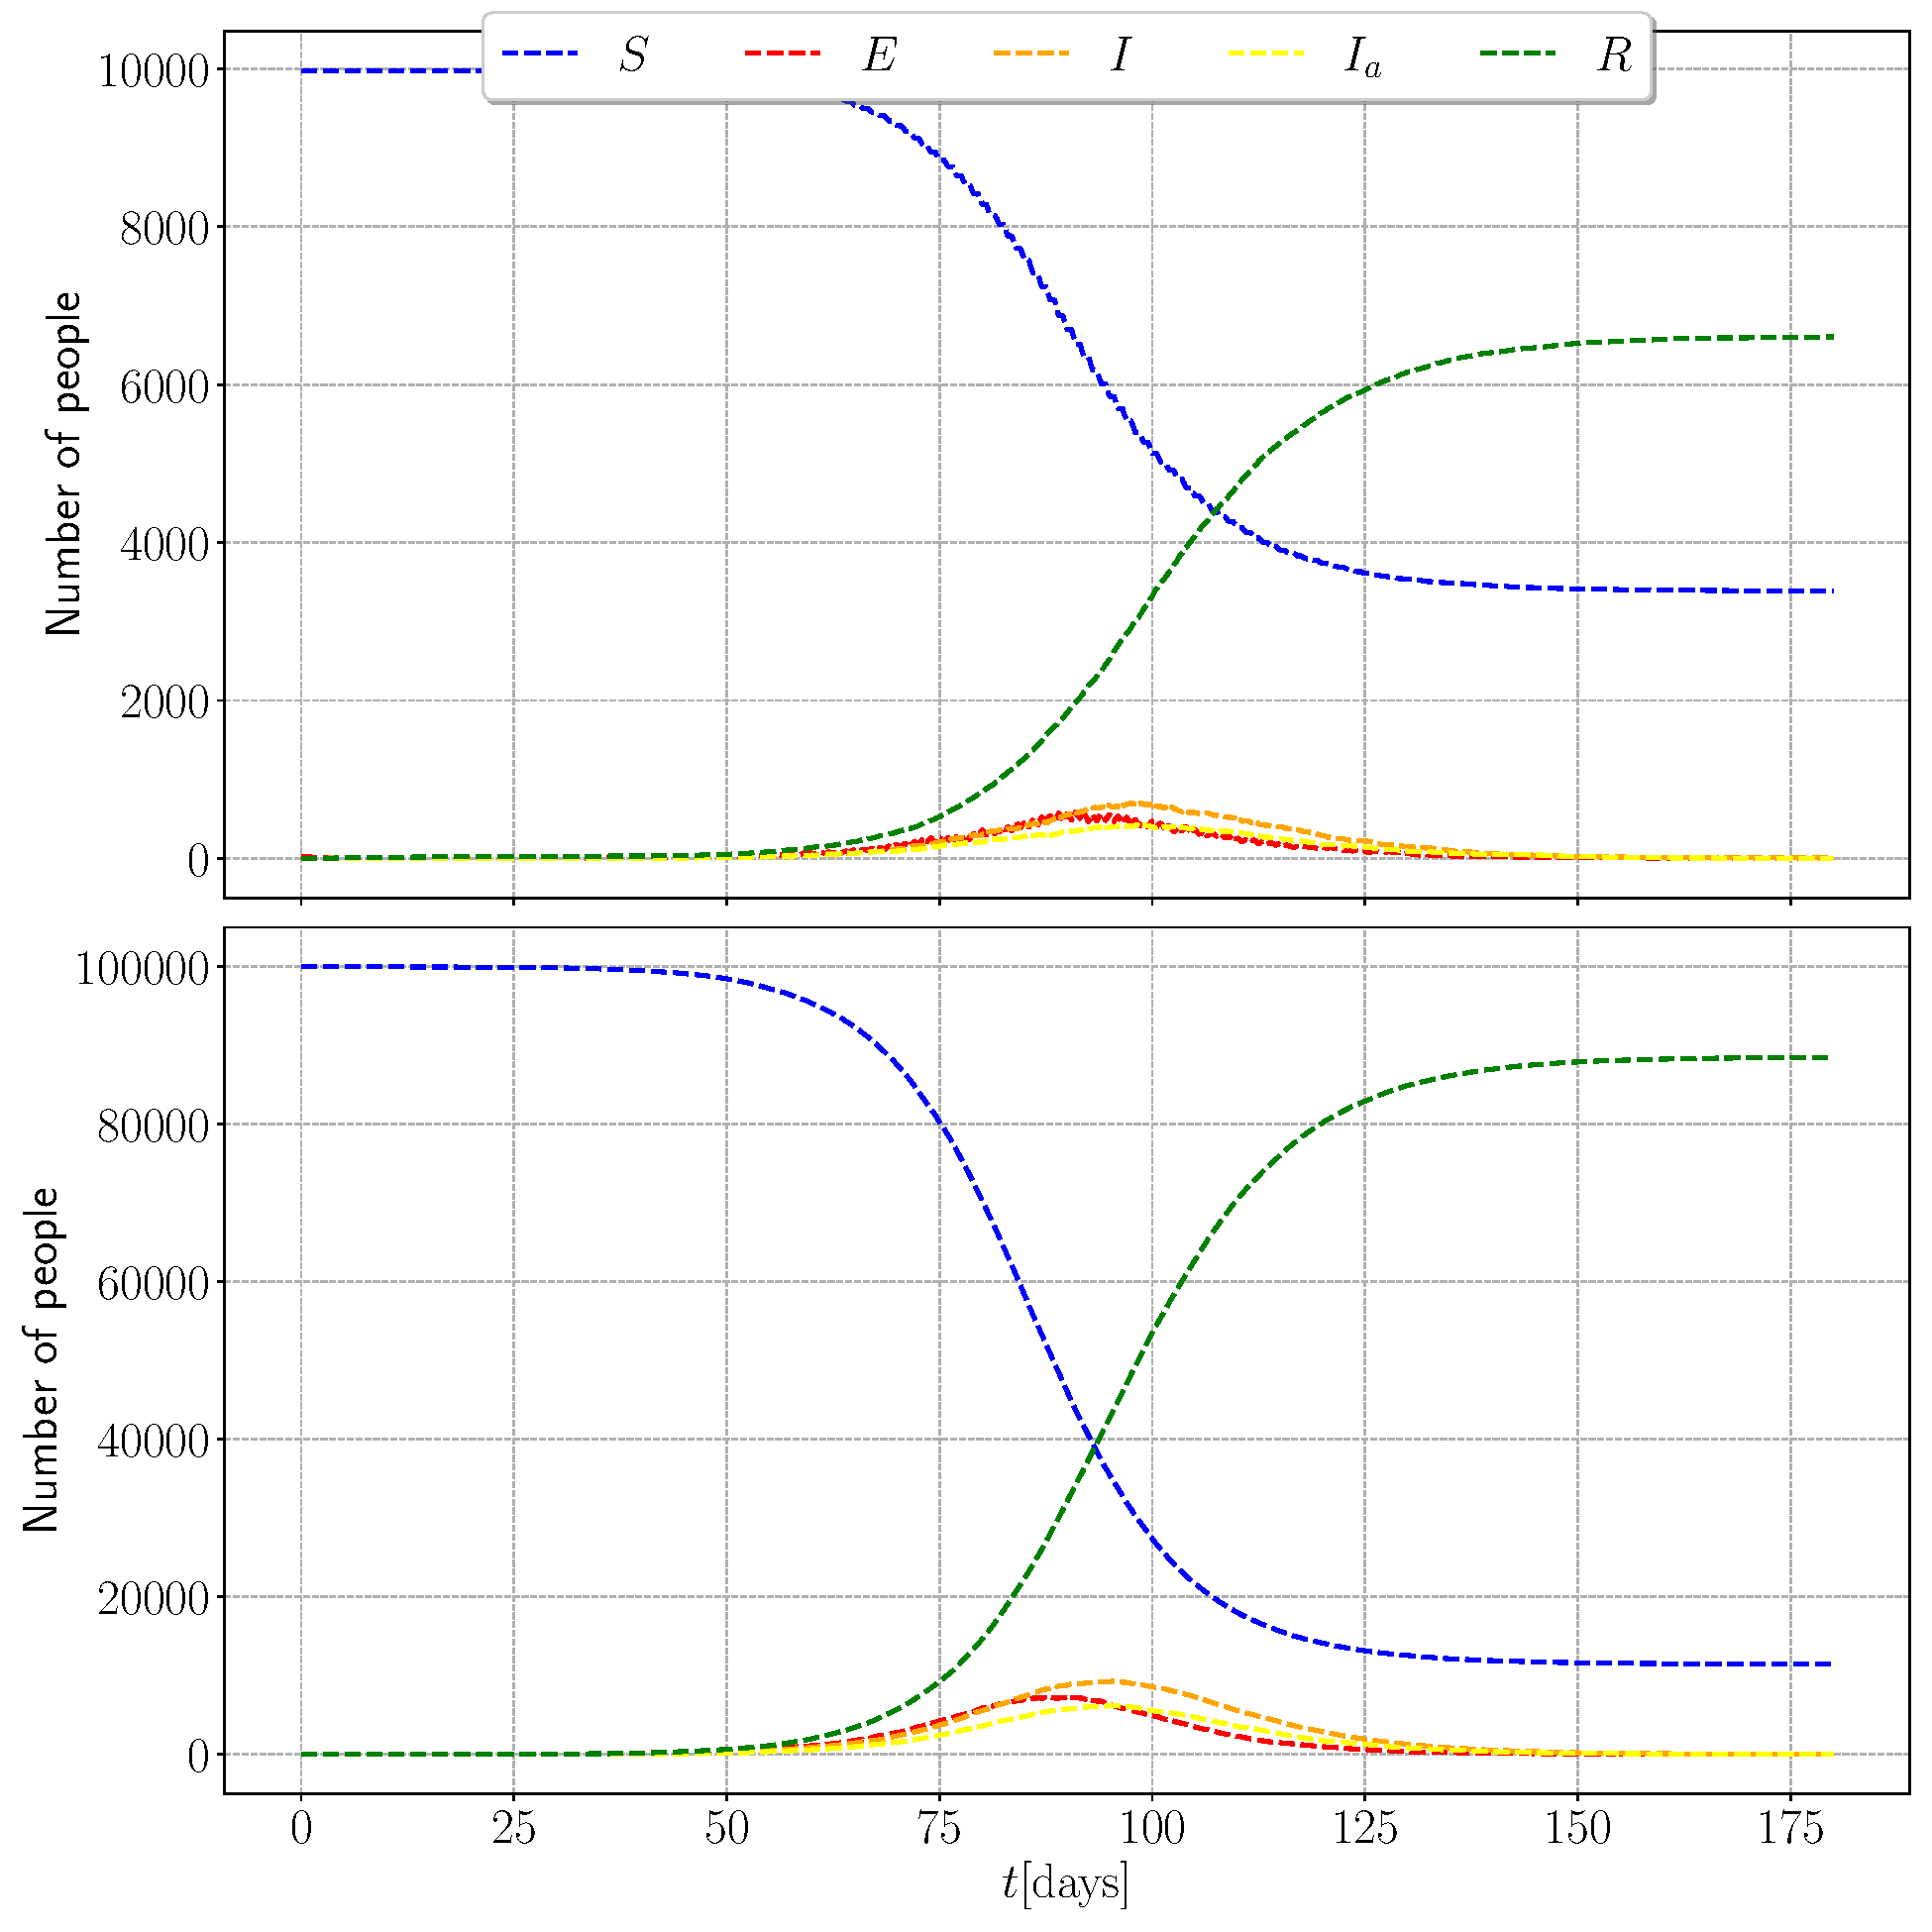
\includegraphics[width=0.6\columnwidth]{../fig/test_commuter_2.pdf}
	\caption{Solutions of Stochastic SEIIaR commuter model for the $2$-city case, with the matrix $\mathbf{\overline{M}}$ in equation \eqref{eq:test_matrix_2}.}
	\label{fig:test_commuter_2}
\end{figure}

\clearpage